\documentclass[a4paper,12pt]{article} % тип документа

% Поля страниц
\usepackage[left=2.5cm,right=2.5cm,
    top=2cm,bottom=2cm,bindingoffset=0cm]{geometry}
    
%Пакет дял таблиц   
\usepackage{multirow} 
    
%Отступ после заголовка    
\usepackage{indentfirst}


% Рисунки
\usepackage{floatrow,graphicx,calc}
\usepackage{wrapfig}

%%% Работа с картинками
\usepackage{graphicx}  % Для вставки рисунков
\graphicspath{{images/}{images2/}}  % папки с картинками
\setlength\fboxsep{3pt} % Отступ рамки \fbox{} от рисунка
\setlength\fboxrule{1pt} % Толщина линий рамки \fbox{}
\usepackage{wrapfig} % Обтекание рисунков и таблиц текстом

% Создаёем новый разделитель
\DeclareFloatSeparators{mysep}{\hspace{1cm}}

% Ссылки?
\usepackage{hyperref}
\usepackage[rgb]{xcolor}
\hypersetup{				% Гиперссылки
    colorlinks=true,       	% false: ссылки в рамках
	urlcolor=blue          % на URL
}


%  Русский язык
\usepackage[T2A]{fontenc}			% кодировка
\usepackage[utf8]{inputenc}			% кодировка исходного текста
\usepackage[english,russian]{babel}	% локализация и переносы




% Математика
\usepackage{amsmath,amsfonts,amssymb,amsthm,mathtools}

%%% Дополнительная работа с математикой
\usepackage{amsmath,amsfonts,amssymb,amsthm,mathtools} % AMS
\usepackage{icomma} % "Умная" запятая: $0,2$ --- число, $0, 2$ --- перечисление


% Что-то 
\usepackage{wasysym}


\begin{document}
\begin{center}
	\footnotesize{ФЕДЕРАЛЬНОЕ ГОСУДАРСТВЕННОЕ АВТОНОМНОЕ ОБРАЗОВАТЕЛЬНОЕ 			УЧРЕЖДЕНИЕ ВЫСШЕГО ОБРАЗОВАНИЯ}\\
	\footnotesize{МОСКОВСКИЙ ФИЗИКО-ТЕХНИЧЕСКИЙ ИНСТИТУТ\\(НАЦИОНАЛЬНЫЙ 			ИССЛЕДОВАТЕЛЬСКИЙ УНИВЕРСИТЕТ)}\\
	\footnotesize{ФАКУЛЬТЕТ ОБЩЕЙ И ПРИКЛАДНОЙ ФИЗИКИ\\}
	\hfill \break
	\hfill \break
	\hfill \break
	\hfill \break
\end{center}


\begin{figure*}[h]
    \centering
    \includegraphics*[width=10cm,height=7cm,keepaspectratio]{mipt_eng_text_png.png}
    \label{fig:my_label}
\end{figure*}


\begin{center}   
    \hfill \break
	\hfill \break
	\hfill \break
	\large{Лабораторная работа № 3.2.8\\ \hfill \break\Large{Релаксационные колебания}}\\
	\hfill \break
	\hfill \break
	\hfill \break
	\hfill \break
	\begin{flushright}
		Баранов Даниил\\
		Группа Б02-103
	\end{flushright}
	\hfill \break
	\hfill \break
	\hfill \break
\end{center}
\hfill \break
\hfill \break
\hfill \break
\hfill \break
\begin{center}
	Долгопрудный, 2022 г.
\end{center}
\thispagestyle{empty}

\newpage

\textbf{Цель работы:} изучение вольтамперной характеристики нормального тлеющего заряда; исследование релаксационного генератора на стабилитроне.

\textbf{В работе используются:} стабилитрон СГ-2 (газонаполненный диод) на монтажной панели, магазин ёмкостей, магазин сопротивлений, источник питания, амперметр, вольтметр, осциллограф.

\section{Теоретические сведения}

 Колебательные системы, как правило, имеют два накопителя, между которыми происходит перекачка энергии. В контуре, содержащем конденсатор и катушку индуктивности, электрическая энергия переходит в магнитную и обратно; при колебаниях маятника потенциальная энергия поля тяжести переходит в кинетическую энергию движущейся массы и т.д. 

\begin{wrapfigure}{r}{0.3\textwidth} 
\begin{center}
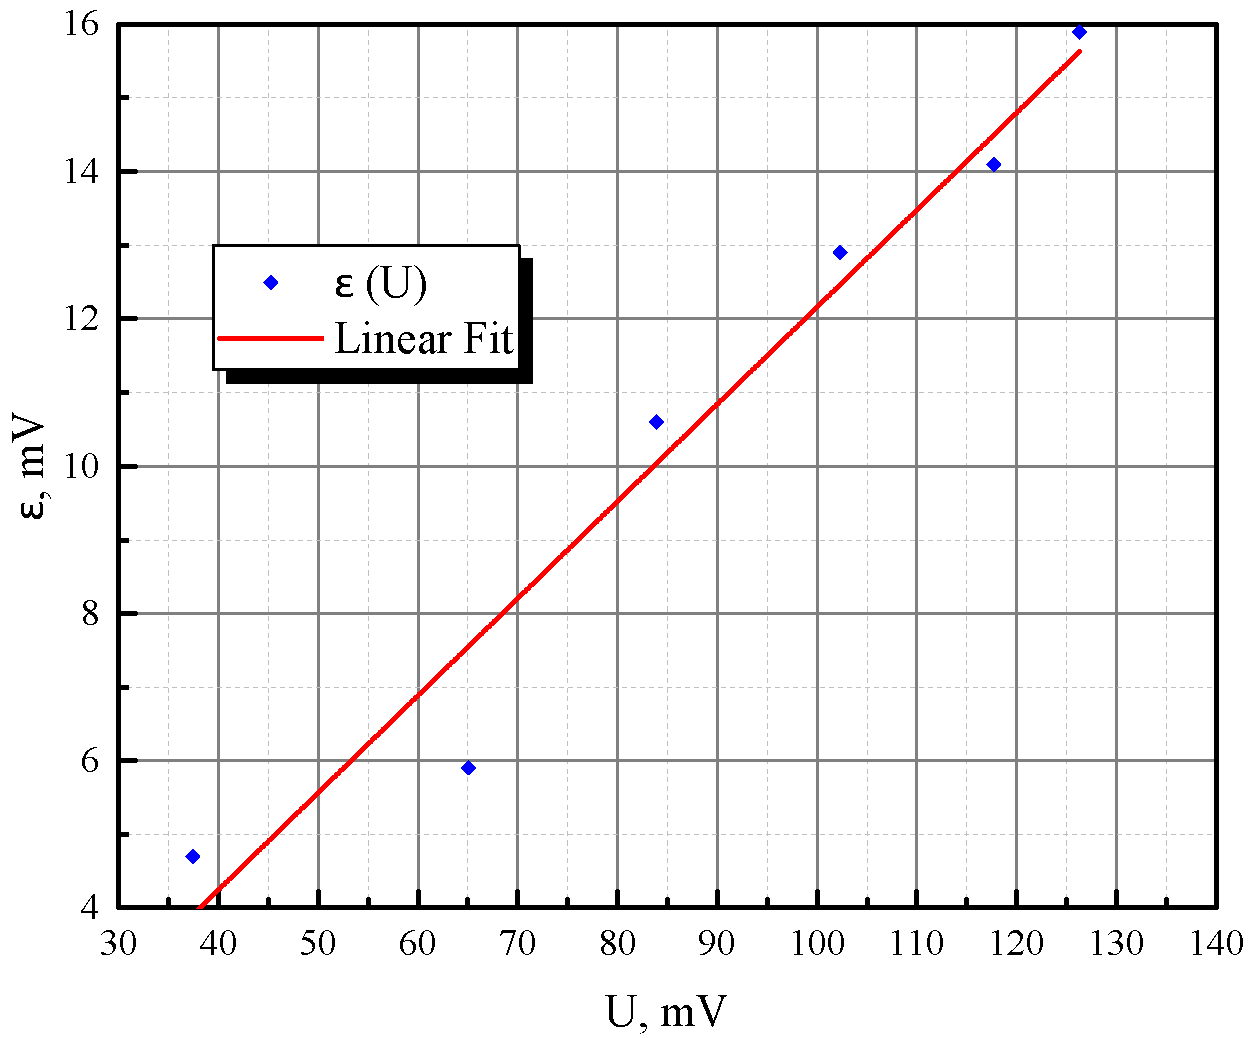
\includegraphics[width=1\textwidth]{3.2.8/graph.jpg} 
\caption{\centering{Вольтамперная характеристика стабилитрона с последовательно включенным резистором}}
\end{center}
\end{wrapfigure}

Встречаются, однако, колебательные системы, содержащие всего один накопитель энергии. Рассмотрим в качестве примера электрическую цепь, содержащую конденсатор и сопротивление без самоиндукции. Разряд конденсатора через сопротивление представляет собой апериодический процесс. Разряду, однако, можно придать периодический характер, возобновляя заряд конденсатора через постоянные промежутки времени. Колебания в этом случае являются совокупностью двух апериодических процессов - процесса зарядки конденсатора и процесса его разрядки. Такие колебания называются релаксационними.\\
В нашей установке роль ключа, обеспечивающего последовательно попеременную зарядку и разрядку конденсатора, играет газоразрядный диод. Зависимость тока от напряжения для газоразрядной лампы не подчиняется закону Ома и характеризуется рядом особенностей (рис. 1). При малых напряжениях лампа не пропускает тока вовсе (не горит). Ток в лампе возникает только в том случае, если разность потенциалов на её электродах достигает напряжения зажигания $V_{1} .$ При этом, тлеюиций разряд. При дальнейшем незначительном увеличении напряжения сила тока заметно возрастает по закону, близкому к линейному. 
Если начать уменьшать напряжение на горящей лампе, то при напряжении, равном $V_{1},$ лампа ещё не гаснет, и сила тока продолжает уменьшаться. Лампа перестанет пропускать ток лишь при напряжении гашения $V_{2},$ которое обычно существенно меньше $V_{1}$. Сила тока при этом скачком падает от значения $I_{2}\left(I_{2}<I_{1}\right)$ до нуля. Характеристика, изображённая на рис. 1, несколько идеализирована. $\mathrm{Y}$ реальной лампы зависимость $I(V)$ не вполне линейна. При $V>V_{1}$ графики
соответствующие возрастанию и убыванию напряжения, не всегда совпадают. Эти отличия, впрочем, носят второстепенный характер и для нашей задачи несущественны.


\begin{wrapfigure}{r}{0.3\textwidth} 
\begin{center}
\includegraphics[width=1\textwidth]{scheme.jpg}
\caption{\centering{Принципиальная схема релаксационного генератора}}
\label{osc}
\end{center}
\end{wrapfigure}

\\

Рассмотрим схему релаксационного генератора, представленную на рис. $2 .$ Пусть напряжение бата- реи $U$ больше напряжения зажигания $V_{1} .$ В обозначениях, принятых на схеме, справедливо уравнение
\begin{equation*}
I(V)=\frac{U-V}{R}
\end{equation*}
\begin{equation}
C \frac{d V}{d T}+I(V)=\frac{U-V}{R}
\end{equation}


В стационарном режиме работы, когда напряжение $V$ на конденсаторе постоянно и $d V / d t=0,$ ток через лампу равен

\begin{equation}
    I_{\mathrm{cr}}=\frac{U-V}{R}
\end{equation}

\begin{wrapfigure}{r}{0.3\textwidth} 
\begin{center}
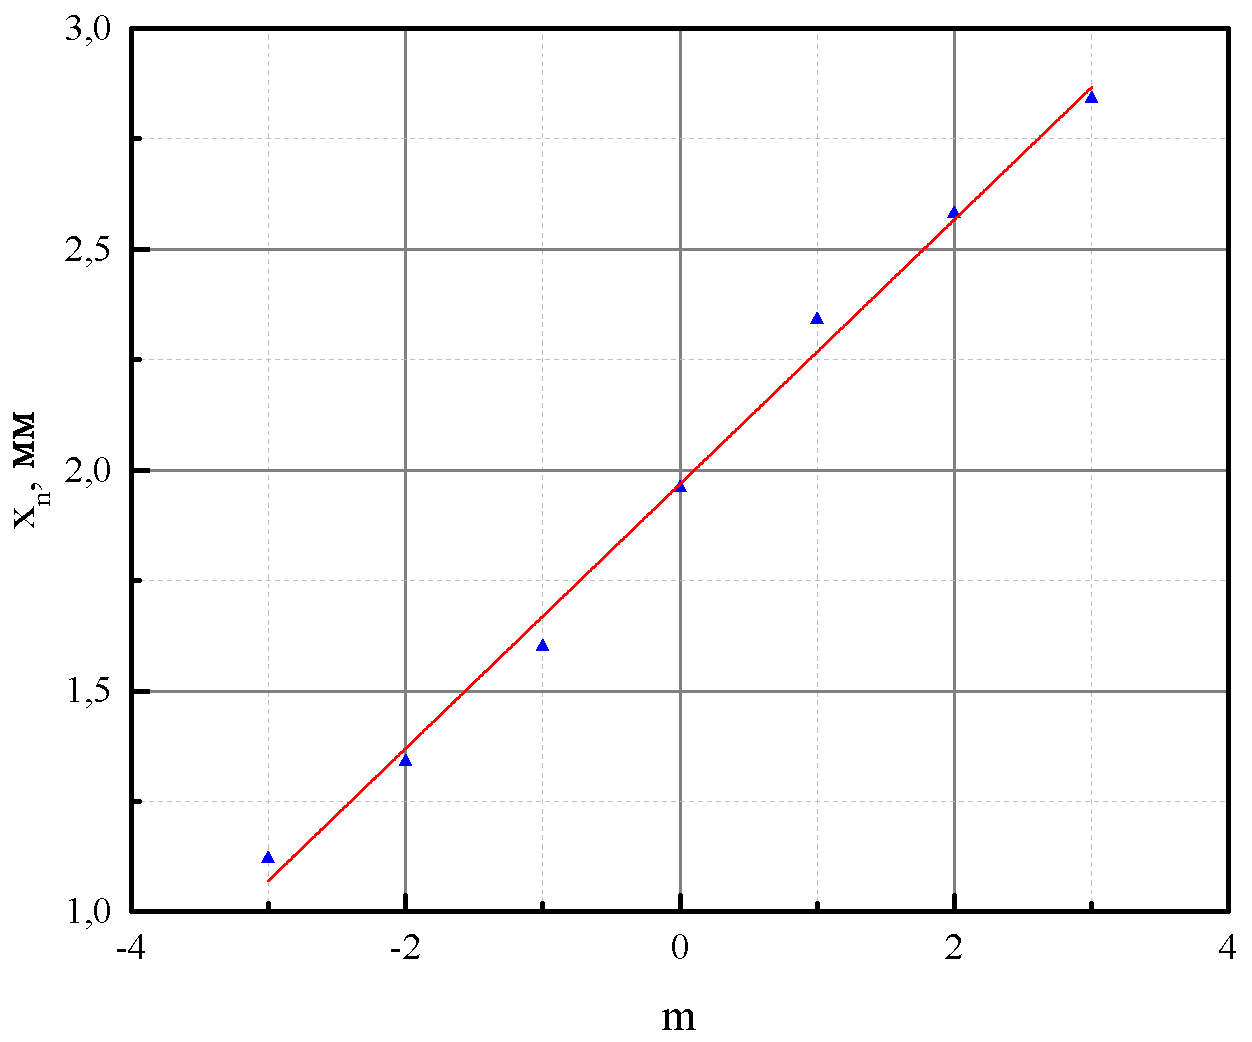
\includegraphics[width=1\textwidth]{3.2.8/graph2.jpg}
\caption{\centering{Режимы работы релаксационного генератора}}
\end{center}
\end{wrapfigure}

Равенство (2) может быть представлено графически (рис. 3) При разных $R$ графрики имеют вид прямых, пересекаЮщихся в точке $V=U, I=0 .$ Область, где эти иагрузочиъе прямвие пересекают вольт-амперную характеристику лампы, соответствует стационарному режиму - при малых $R$ (прямая 1$)$ лампа горит постоянно, колебания Отсутствуют. Прямая $2,$ проходящая через точку $\left(I_{2}, V_{2}\right),$ соответствует критическому сопротивлению

\begin{equation}
R_{\mathrm{Kp}}=\frac{U-V_{2}}{I_{2}}
\end{equation}

При сопротивлении $R>R_{\text {кр }}$ нагрузочная прямая $3 \quad$ не пересекает характеристику лампы, поэтому стационарный режим невозможен. В этом случае в системе устанавливаются колебания. Рассмотрим, как происходит колебательный процесс. Пусть в начале опыта ключ К разомкнут (рис. 2) и $V=0 .$ Замкнём ключ. Конденсатор $C$ начинает заряжаться через сопротивление $R,$ напряжение на нём увеличивается (рис. 4) Как только оно достигнет напряжения зажигания $V_{1},$ лампа начинает проводить ток, причём прохождение тока сопровождается разрядкой конденсатора. В самом деле, батарея $U,$ подключённая через большое сопротивление $R,$ не может поддерживать необходимую для горения лампы величину тока. Во время горения лампы конденсатор разряжается, и когда напряжение на нём достигнет потенциала гашения, лампа перестанет проводить ток, а конденсатор вновь начнёт заряжаться. Возникают релаксационные колебания с амплитудой, равной $\left(V_{1}-V_{2}\right) .$

\begin{wrapfigure}{r}{0.3\textwidth} 
\begin{center}
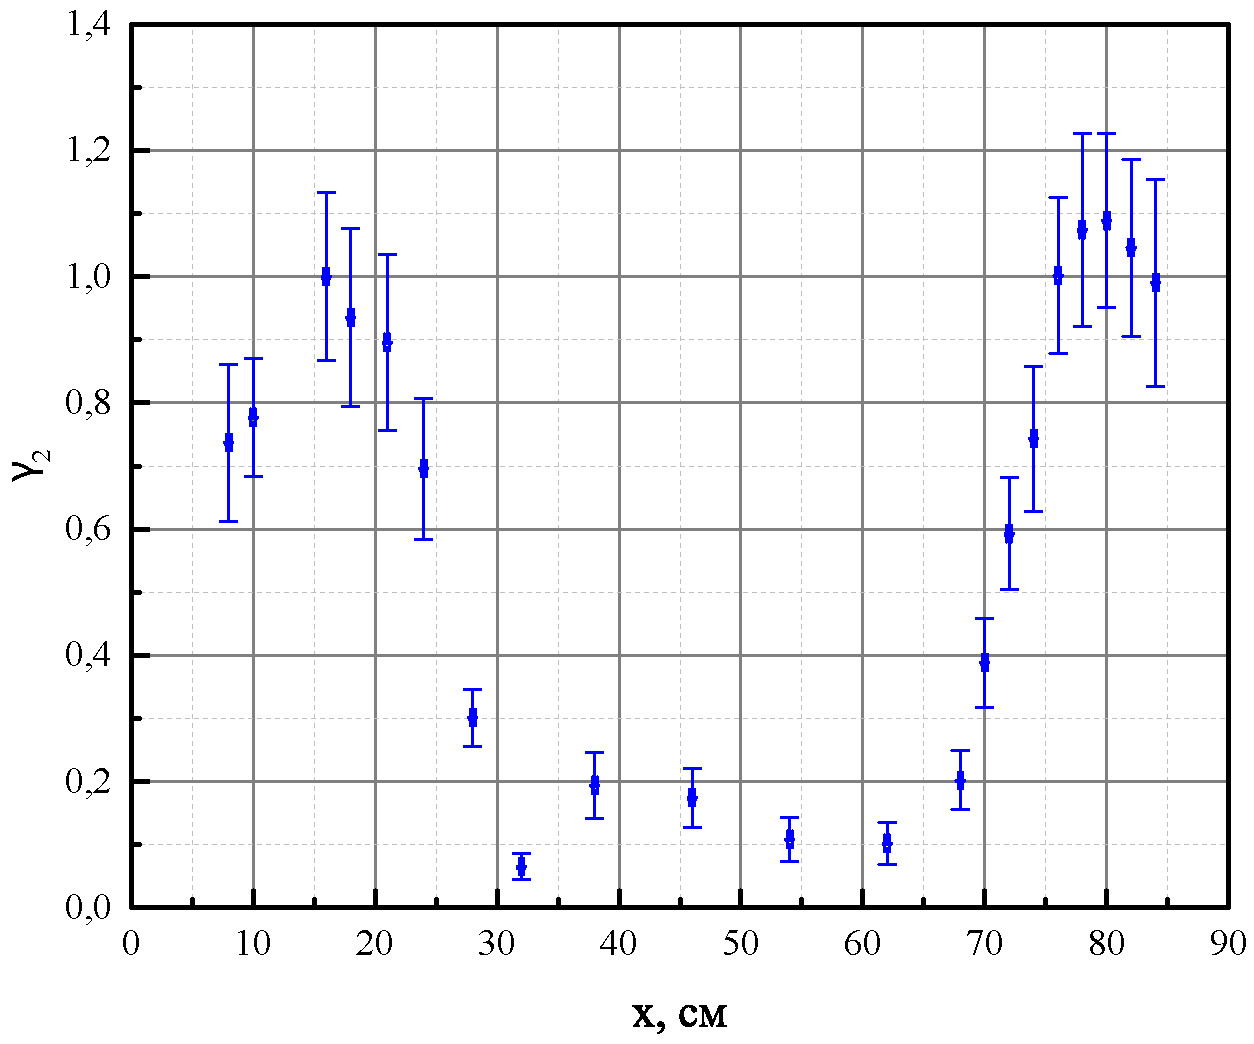
\includegraphics[width=1\textwidth]{3.2.8/graph3.jpg}
\caption{\centering{Осциллограмма релаксационных колебаний}}
\end{center}
\end{wrapfigure}

Рассчитаем период колебаний. Полное время одного периода колебаний Т состоит из суммы времени зарядки $\tau_{3}$ и времени разрядки $\tau_{\mathrm{p}},$ но если сопротивление $R$ существенно превосходит сопротивление Зажжённой лампы, то $\tau_{3} \gg \tau_{\mathrm{p}}$ и $T \simeq \tau_{3}($ этим случаем мы и ограничимся). Во время зарядки конденсатора лампа не горит $[I(V)=0],$ и уравнение (1) приобретает вид
\begin{equation}
R C \frac{d V}{d t}=U-V    
\end{equation}

Будем отсчитывать время с момента гашения лампы, так что $V=V_{2}$ при $t=0$ (рис. 4$) .$ Решив уравнение $(4),$ найдём
\begin{equation}
 V=U-\left(U-V_{2}\right) e^{-t /(R C)}   
\end{equation}


$\mathrm{B}$ момент зажигания $t=\tau_{3}, V=V_{1},$ поэтому
\begin{equation}
V_{1}=U-\left(U-V_{2}\right) e^{-\tau_{3} /(R C)}
\end{equation}
Из уравнений (5) и (6) нетрудно найти период колебаний:
$$
T \approx \tau_{3}=R C \ln \frac{U-V_{2}}{U-V_{1}}
$$
Развитая выше теория является приближённой. Ряд принятых при расчётах упрощающих предположений оговорен в тексте. Следует иметь в виду, что мы полностью пренебрегли паразитными емкостями и индуктивностями схемы. Не
рассматривались также процессы развития разряда и деионизация при гашении. Поэтому теория справедлива лишь в тех случаях, когда в схеме установлена достаточно большая ёмкость и когда период колебаний существенно больше времени развития разряда и времени деионизации (практически $\gg 10^{-5}$ с). Кроме того, потенциал гашения $V_{2},$ взятый из статической вольт-амперной характеристики, может отличаться от потенциала гашения лампы, работающей в динамическом режиме релаксационных колебаний.

\section{Результаты измерений и обработка данных}


\subsection{Характеристика стабилитрона}

\begin{wrapfigure}{r}{0.3\textwidth} 
\begin{center}
\includegraphics[width=1.3\textwidth]{3.2.8/scheme2.jpg}
\caption{\centering{Схема установки для изучения характеристик стабилитрона}}
\label{scheme}
\end{center}
\end{wrapfigure}

В первой части работы использовалась схема, изображённая на рис. \ref{scheme}. Добавочное сопротивление $r = 5,1$ кOм было подпаяно между ножкой лампы и соответствующей клеммой для того, чтобы предохранить стабилитрон от перегорания. Это сопротивление оставалось включённым при всех измерениях. 

Вольтамперная характеристика стабилитрона с резистором $r$ при возрастании и убывании напряжения представлена в табл. \ref{voltamp}. При этом, для более точного определения потенциалов зажигания и гашения показания приборов были сняты пятикратно. Потенциалы зажигания ($V_1$) и гашения ($V_2$) отмечены соответсутющими значками в первом столбце.
\hfill \break
\hfill \break

\floatsetup[table]{capposition=top}
\begin{table}[h]
    \centering
    \begin{tabular}{|p{0.5cm}|p{2cm}|p{2cm}|p{2cm}|p{2cm}|}
    \hline & \centering{$V$,В} & \centering{$I$, мА} & \centering{$\sigma_V$, В} & \centering{$\sigma_I$, мА} & 
\hline  \multicolumn{5}{|c|}{Увеличение напряжения} \\ \hline
    $V_1$   & 87,5  & 2,94 & 0,5 & 0,05  \\ \hline
            & 92,6  & 3,93 & 0,5 & 0,05  \\ \hline
            & 100,0 & 5,30 & 0,5 & 0,05  \\ \hline
            & 110,2 & 7,14 & 0,5 & 0,05  \\ \hline
            & 120,0 & 9,23 & 0,5 & 0,05  \\ \hline
            & 130,2 & 11,1 & 0,5 & 0,05  \\ \hline
            & 143,0 & 13,5 & 0,5 & 0,05  \\ \hline
            & 158,0 & 16,4 & 0,5 & 0,05  \\ \hline
           \multicolumn{5}{|c|}{Понижение напряжения} \\ \hline
        & 148,5 & 14,6 & 0,5 & 0,05  \\ \hline 
        & 136,7 & 12,4 & 0,5 & 0,05  \\ \hline 
        & 123,5 & 9,90 & 0,5 & 0,05  \\ \hline 
        & 108,7 & 6,90 & 0,5 & 0,05  \\ \hline 
        & 95,3  & 4,56 & 0,5 & 0,05  \\ \hline 
        & 84,5  & 2,47 & 0,5 & 0,05  \\ \hline 
$V_2$   & 81,6  & 0    & 0,5 & 0,05  \\ \hline 
            \multicolumn{5}{|c|}{Повторение измерений} \\ \hline
    $V_1$   & 88,3 & -- & 0,5 & 0,05  \\ \hline
    $V_1$   & 88,0 & -- & 0,5 & 0,05  \\ \hline
    $V_1$   & 87,8 & -- & 0,5 & 0,05  \\ \hline
    $V_2$   & 82,3 & -- & 0,5 & 0,05  \\ \hline
    $V_2$   & 82,0 & -- & 0,5 & 0,05  \\ \hline
    $V_2$   & 83,6 & -- & 0,5 & 0,05  \\ \hline
    \end{tabular}
    \caption{Вольтамперная характеристика стабилитрона}
    \label{voltamp}
\end{table}

По полученным данным был построен график (рис. \ref{iu}). В качестве напряжений зажигания и гашения были взяты средние значения всех измеренний данных величин.

\begin{figure}[h]
    \centering
    \includegraphics[scale=0.7]{3.2.8/I(U).pdf}
    \caption{График зависимости $I(U)$}
    \label{iu}
\end{figure}


\subsection{Осциллограммы релаксационных колебаний}

Для снятия осциллограмм была собрана схема согласно рис. \ref{osc}.
Для проведения эксперимента было выставлено напряжение $U = 117,3 \pm 0,5 $В.\\
После подбора частоты развёртки ЭO, при которой на экране видна картина пилообразных колебаний, было оцененно отношение $\displaystyle \frac{\tau_\text{з}}{\tau_\text{р}}$, которое составило $\approx 15$.\\

При данном значении напряжение $R_\text{кр}$ оказалось равным $140 \pm 1$ кОм. 

Далее была проведена серия измерений для снятия показаний для зависимости $T(C)$. Напряжение при этом было выставлено $118 \pm 0,3 $В, сопротивление -- $R = 560$ кОм. Результаты измерений приведены в таблице \ref{tec}.


\begin{table}[h]
    \centering
    \begin{tabular}{|p{3.5cm}|p{3.5cm}|}
    \hline        $C$, нФ & $T$, мс ($\varepsilon_T = 5\%$) \\ \hline
        50 & 26   \\ \hline
        40 & 21   \\ \hline
        30 & 15,5 \\ \hline
        20 & 10   \\ \hline
        15 & 7,2  \\ \hline
        10 & 4,6  \\ \hline
        5  & 2    \\ \hline 
    \end{tabular}
    \caption{Зависимость периода от электроёмкости (данные)}
    \label{tec}
\end{table}

Данные были нанесены на график (рис. \ref{tc}). Помимо этого, были рассчитаные теоретические значения периода и также отмечены на графике.

\begin{figure}
    \centering
    \includegraphics[scale=0.65]{3.2.8/T(C).pdf}
    \caption{Зависимость времени колебаний от электроёмкости конденсатора}
    \label{tc}
\end{figure}


Как видно из графика, коэффициенты наклона сильно отличаются, из чего следует, что динамический потенциал отличается от статического. Динамический потенциал гашения лампы составил $\approx 42$ В.

\section{Выводы}

Была изучена вольтамперная характеристика нормального тлеющего заряда, и исследован релаксационный генератор на стабилитроне.




\end{document}
